\documentclass[a4paper,12pt]{article}
\usepackage[utf8]{ inputenc}
\usepackage[ngerman]{babel}
\usepackage[a4paper, left=2.5cm, right=2.5cm]{geometry}
\usepackage{graphicx}
\usepackage{subcaption}
\usepackage{fancyhdr}
\usepackage{pdfpages}
\usepackage{listings}
\usepackage{float}

\pagestyle{fancy}
\lstset{
	language=Matlab,
	breaklines=true,
	morekeywords={matlab2tikz},
	keywordstyle=\color{blue},
	morekeywords=[2]{1}, keywordstyle=[2]{\color{black}},
	identifierstyle=\color{black},
	stringstyle=\color{mylilas},
	commentstyle=\color{mygreen},
	showstringspaces=false,
	mathescape=true
	emph=[1]{for,end,break},emphstyle=[1]\color{red},
}

\lhead{Sonneneinstrahlung und Photovoltaik Teil 2}
\chead{}
\rhead{Gruppe D}

\begin{document}
	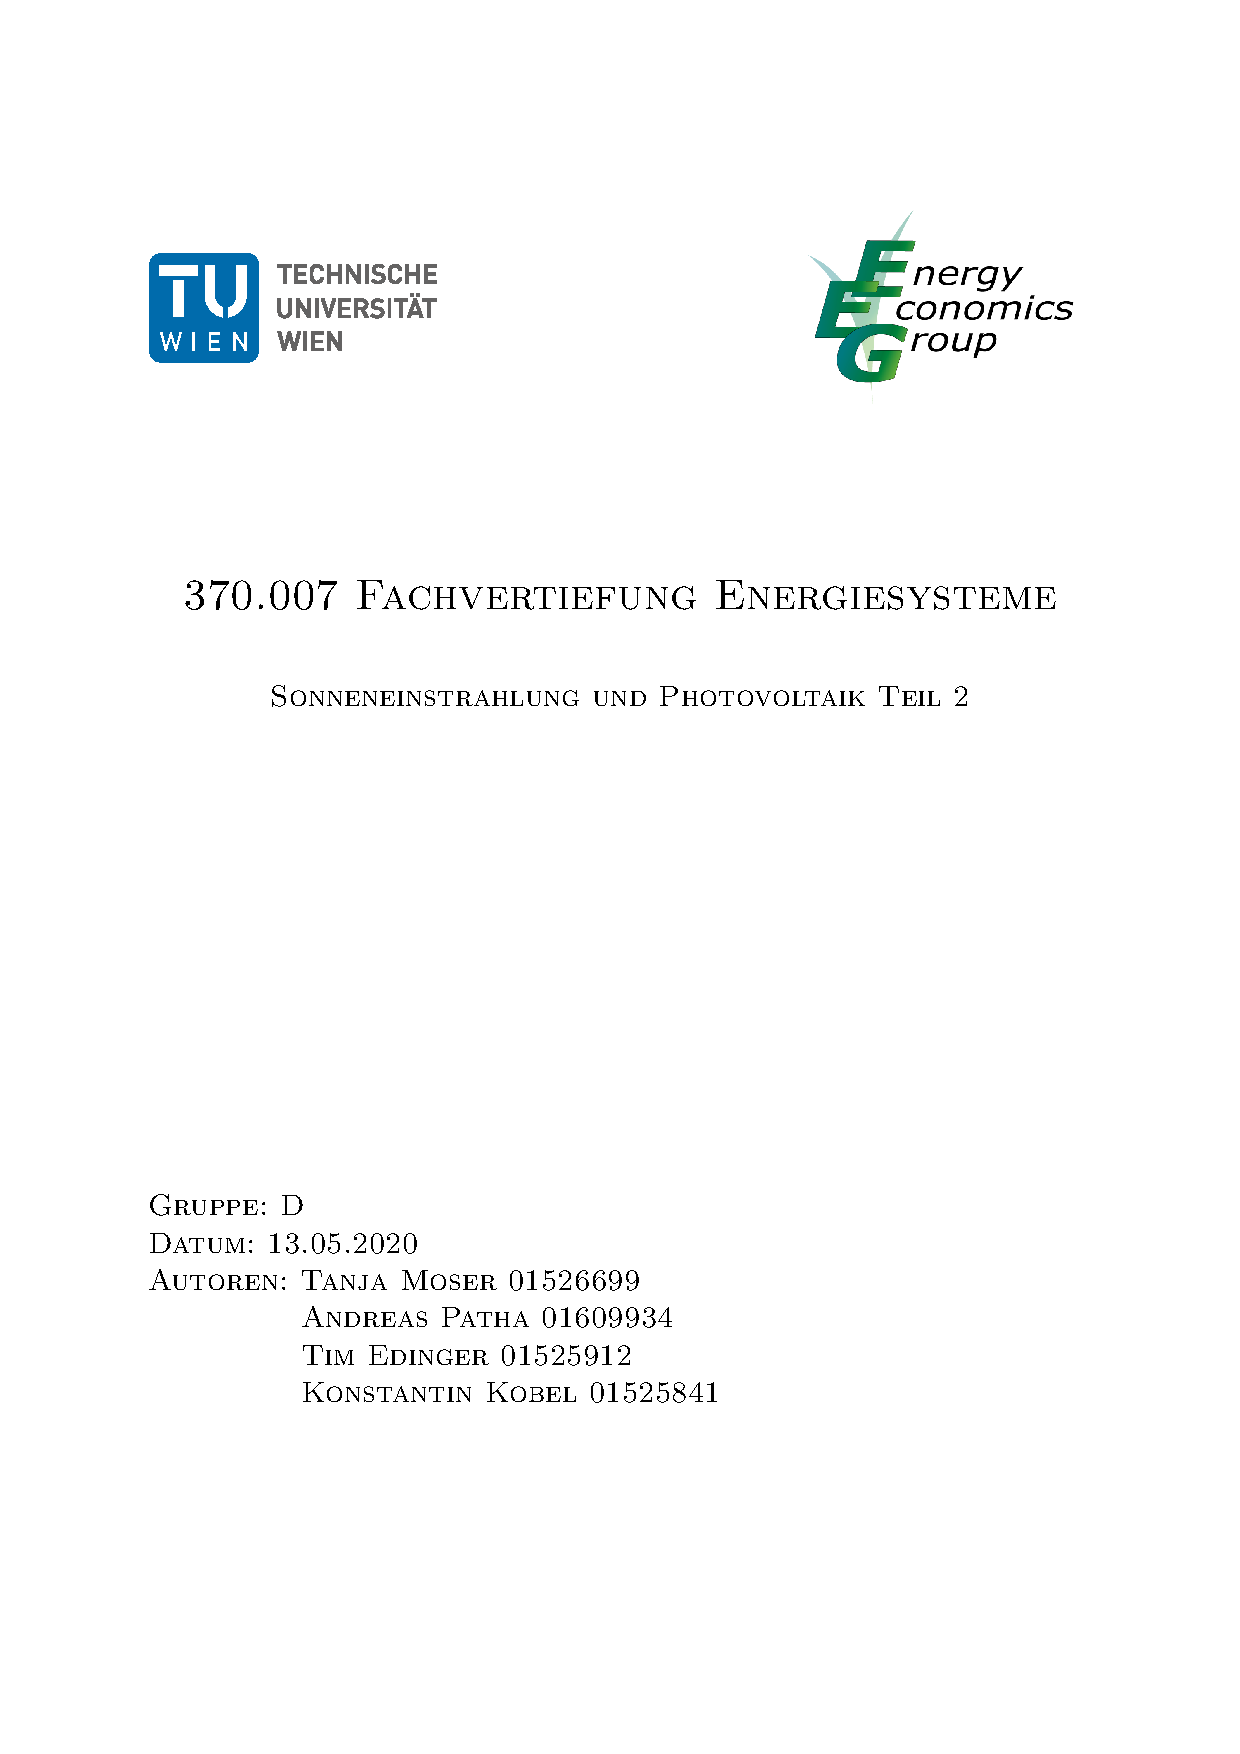
\includepdf{Protokoll_titlepage.pdf}
	
	\newpage
	%Inhaltsverzeichnis
	\tableofcontents
	
	\newpage
	\section{Aufgabenstellung}
	\subsection{Aufgabe 2.1}
	Aufgabe 2.1 befasst sich mit einer PV-Anlage der ersten Übung, unter Einfluss der Temperatur und Einstrahlung mit folgenden Parametern:
	\begin{itemize}
		% Wusste nicht ob ihr die Angaben von dem ersten Protokoll nochmal drin stehen haben wollt!
		%\item Der Standort ist Wien ($48.2^{\circ}$N, $16.3^{\circ}$O).
		%\item Die installierte Leistung ist $1kWp$.
		%\item Der Neigungswinkel der PV-Anlage beträgt $20^{\circ}$.
		%\item Der Azimut der Anlage ist $180^{\circ}$ Süden.
		%\item Die Zeit in Viertelstunden-Werten ist in der Datei $time.mat$ gegeben.\item Anlage am Dach - gut belüftet $c_{T}$ mit dem Wert $0.426$ (für Gelichung 3)
		\item Sonstige Verluste $\eta_{sonst}$ (Reflexion, Temperatur, Wechselrichter, etc.) werden mit dem Wert $0.8$ eingerechnet.				\item Der Modulwirkungsgrad $\eta_{Modul}$ ist $0.17$.
		\item Silizium-Zelle: Koeffizienten $kx, x = 1, ... , 6$ (Huld et al.-Table1 -S.329)
		\item Die Errechnung des Sonnenstandes erfolgt mit der in der Datei $SonnenstandTST.m$ (zur Verfügung gestellten Funktion $SonnenstandTST()$ 	)				\item Die Strahlungsdaten für den Standort sind in der Datei $Strahlung.mat$ gegeben.
		\item Die Daten zur Temperatur sind in der Datei $Temperatur.mat$ gegeben.
	\end{itemize}
	Die Aufgaben lauten:
	\begin{itemize}
		\item[a)] Erweitern Sie das Modell, um die Berücksichtigung des Einflusses der Temperatur und der
Einstrahlung auf den Wirkungsgrad des PV-Moduls (erweitern Sie Ihre Funktion aus
Aufgabe 1.1).
		\item[b)] Vergleichen Sie Ihre Ergebnisse mit jenen aus Aufgabe 1. Wie verändert sich die Verteilung
der Erzeugung über die Jahreszeiten und innerhalb des Tages im Vergleich zum
vereinfachten Ansatz ohne Berücksichtigung von Temperatur- und Strahlungseinfluss auf
den Wirkungsgrad? Stellen Sie dazu die monatlichen Erträge gegenüber sowie die
durchschnittlichen stündlichen Werte.
	\end{itemize}
	\subsection{Aufgabe 2.2}
	Die Unterpunkte der Aufgabe 2.2 lauten:
	\begin{itemize}
		\item[a)] Berechnen Sie die Erzeugung einer 1 kWpeak Anlage (in Wien) unter Abhängigkeit
des Aufstellwinkels (mit Temperatureinfluss). Variieren Sie den Neigungswinkel
der Anlage von $0$ bis $90$ in $2.5$-Intervallen und den Azimut der Anlage von $0$ bis
$360$ in $10$-Schritten.
		\item[b)] Stellen Sie die Volllaststunden der Anlage in Abhängigkeit der Aufstellwinkel in
einer 3D-Grafik dar. Verwenden Sie dazu einmal die Plot-Funktion meshc und
einmal contour, um ISO-Ertragslinien darzustellen.
\begin{itemize}
\item Bei welcher Winkelkombination erhalten Sie den höchsten Ertrag?
\item Zeichnen Sie diesen Punkt in den beiden Darstellungen ein!
\end{itemize}
		\item[c)] Wiederholen Sie die 3D-Berechnung und Darstellung einmal für den Monat Juni
und einmal für Dezember.
\begin{itemize}
\item Was beobachten Sie?
\item Welche Winkelkombinationen würden Sie für die diese beiden Monate empfehlen?
\end{itemize}
	\end{itemize}
	\subsection{Aufgabe 2.3}
	Vergleichen Sie die Erzeugung einer 1 kWpeak Anlage von 2 zusätzlichen (möglichst
unterschiedlichen) Standorten in Europa mit der von Wien. Die Strahlungs- und
Temperaturdaten sind für das Jahr 2005 auf
http://www.soda-pro.com/web-services/radiation/helioclim-3-archives-for-free verfügbar.
	\begin{itemize}
		\item[a)]Vergleichen Sie die Erzeugung der Standorte und zeigen Sie die wesentlichen
Unterschiede zwischen den Standorten:
\begin{itemize}
\item gesamte Jahreserzeugung und Volllaststunden
\item durchschnittliche Tagesproduktion ( 24 Werte pro Standort)
\end{itemize}
	\item[b)] Stellen Sie die Volllaststunden der Anlagen in Abhängigkeit der Aufstellwinkel in
einer Grafik dar. Welche Unterschiede erkennen Sie? Wo liegen jeweils die
optimalen Winkelkombinationen für jeden Standort?
	\item[c)] Beschreiben Sie die Gründe, warum die Erzeugung aus PV-Anlagen an
unterschiedlichen Standorten zeitliche (tageszeitliche und saisonale) Unterschiede
aufweist.
	\end{itemize}
	\newpage
	\section{Berechnungen}
	\subsection{Temperaturabhängigkeit einer PV-Anlage}
	Wie bereits in Kapitel 5 "Interpretation der Ergebnisse" von Protokoll 1 erwähnt, ist der Wirkungsgrad einer PV-Anlage von der Temperatur dieser abhängig. Generell gilt, dass der Wirkungsgrad bei niedrigen Temperaturen steigt und bei hohen Temperaturen sinkt.\newline
	Der temperaturabhängige Wirkungsgrad kann über folgende Formel ermittelt werden:
	\begin{equation}
	\eta_{rel}=1+k_1*\ln{(G')}+k_2*\ln{(G')}^2+T'*(k_3+k_4*\ln{(G')}+k_5*\ln{(G')}^2)+k_6*T'^2
	\end{equation}
	Die Parameter in dieser Gleichung sind folgendermaßen definiert:
	\begin{itemize}
		\item \textbf{$G$} - Dieser Wert entspricht der gesamten, auf die PV-Anlage auftreffenden, Einstrahlung. (Die Berechnung von $G$ wird im ersten Protokoll erklärt.)
		\item \textbf{$T_{mod_{STC}}$} - Dieser Wert wurde als Referenzwert, für die Temperatur des Moduls, in den Standard Test Conditions definiert. Er entspricht $25^{\circ}C$.
		\item \textbf{$G_{STC}$} - Dieser Wert wurde in den Standard Test Conditions als Referenzwert für die einfallende Strahlung definiert. Er entspricht $1000W/m^2$.
		\item \textbf{$c_T$} - Dieser Faktor gibt an, wie stark sich das Modul durch Sonneneinstrahlung erhitzt.
		\item \textbf{$T_{amb}$} - Entspricht der Umgebungstemperatur der PV-Anlage.
		\item \textbf{$T_{mod}$} - Entspricht der tatsächlichen Temperatur des Moduls. Diese errechnet sich zu $T_{amb}+c_T*G$.
		\item \textbf{$G'$} - Dieser Wert ist der Quotient aus der tatsächlichen Einstrahlung $G$ und der in den Standard Test Conditions definierten Einstrahlung $G_{STC}$. Daraus ergibt sich $G'=\frac{G}{G_{STC}}$.
		\item \textbf{$T'$} - Die Temperatur des Moduls wird als Differenz zum Referenzwert $T_{mod_{STC}}$ angegeben. Diese errechnet sich zu $T'=T_{mod}-T_{mod_{STC}}$.
	\end{itemize}
	Die Parameter $k_1$ bis $k_6$, für c-Si Module, müssen durch Messungen gefunden werden. Sie werden im Skript $Mapping the performance of PV modules, effects of module type and data averaging$ folgendermaßen definiert:
	\begin{table}[H]
		\centering
		\begin{tabular}{|l|c|c|c|c|c|}
			\hline
			\multicolumn{1}{|c|}{$k_1$} & $k_2$     & $k_3$     & $k_4$    & $k_5$    & $k_6$    \\ \hline
			-0.017162                   & -0.040289 & -0.004681 & 0.000148 & 0.000169 & 0.000005 \\ \hline
		\end{tabular}
	\end{table}
	In MATLAB ergibt sich daraus folgender Code:
	\begin{lstlisting}
	Tmod = repelem(Temperatur,4) + ct.*GesGen;
	T = Tmod $-$ TmodSTC;
	TWirkungsgrad=1+k1.*log(G)+k2.*pow2(log(G))+T.*(k3+k4.*log(G)+k5.*pow2(log(G)))+k6.*pow2(T);
	\end{lstlisting}
	Da die Temperatur in der Datei $Temperatur.mat$ nur in Stunden-Intervallen gegeben ist, müssen wir den Array der Temperatur dementsprechend skalieren, damit eine Multiplikation mit $GesGen$ möglich ist. ($GesGen$ enthält Viertelstunden-Werte)\newline
	Die Berechnung von $GesGen$ wird im ersten Protokoll erklärt.\newline
	Daraus ergibt sich die temperaturabhängige Energie zu
	\begin{equation}
	E=E_{G,gen}*A*\eta_{Modul}*\eta_{sonst}*\eta_{rel}
	\end{equation}
	Definitionen zu Formel (2) können dem ersten Protokoll entnommen werden.
	\newpage	
	\section{Ergebnisse - Aufgabe 2.1}
	\subsection{2.1.a}
	In Aufgabe 2.1.a ging es darum das Modell aus Aufgabe 1.1.a, aus dem ersten Protokoll, so zu erweitern, dass die Temperaturabhängigkeit der PV-Anlage in den Berechnungen berücksichtigt wird.\newline
	Das Modell zur Berechnung des temperaturabhängigen Ertrags befindet sich in der Datei $Beispiel2.m$ bzw. in $Jahreserzeugung.m$. Die Ergebnisse der Berechnungen werden im Unterpunkt 2.1.b beschrieben. 
	\subsection{2.1.b}
	In Aufgabe 2.1.b ging es darum zu demonstrieren, wie sich die Verteilung der Erzeugung über die Jahreszeiten und innerhalb des Tages verändert, wenn die Temperaturabhängigkeit der PV-Anlage in den Berechnungen berücksichtigt wird.\newline
	\begin{figure}[H]
		\centering
		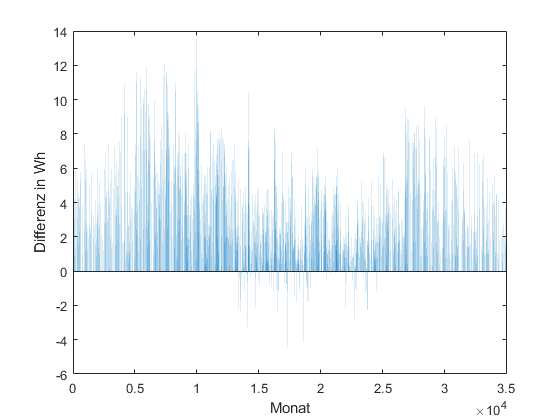
\includegraphics[width=12cm]{img/results/DifferenzIdealTemp}
		\caption{Differenz zwischen dem idealen und dem temperaturabhängigen Ertrag, über das Jahr 2005. (in Viertelstunden-Intervallen)}
	\end{figure}
	In Abbildung 1 ist die Differenz zwischen dem idealen und dem temperaturabhängigen Ertrag dargestellt. Für jeden Viertelstunden-Wert des Jahres 2005 wurde die Differenz errechnet und dann in einem Balkendiagramm dargestellt.\newline
	In MATLAB wurde das Diagramm mit folgendem Code erstellt:
	\begin{lstlisting}
	bar(EgesT$-$Eges)
	\end{lstlisting}
	$Eges$ entspricht dem idealen und $EgesT$ dem temperaturabhängigen Ertrag.\newline
	Im Diagramm ist zu erkennen, dass der temperaturabhängige Ertrag in den Monaten von Jänner bis Mai, sowie von Oktober bis Dezember, deutlich höher ist, als der ideale Ertrag. Der Grund dafür ist der erhöhte Wirkungsgrad der PV-Anlage bei niedrigeren Temperaturen.\newline
	In den Sommer-Monaten, von Juni bis September, ist die Tempertature hoch, woraus ein niedrigerer Wirkungsgrad der PV-Anlage resultiert. Das hat wiederum zur Folge, dass in diesen Monaten das temperaturabhängige Modell vereinzelt einen niedrigeren Ertrag liefert, als die ideale Berechnung. \\ \par Zur besseren Darstellung der Veränderung sollten in Aufgabe 2.1.b zusätzlich die monatlichen Erträge sowie die durchschnittlichen stündlichen Werte gegenüber gestellt werden.\\ \par
	\begin{figure}[H]
		\centering
		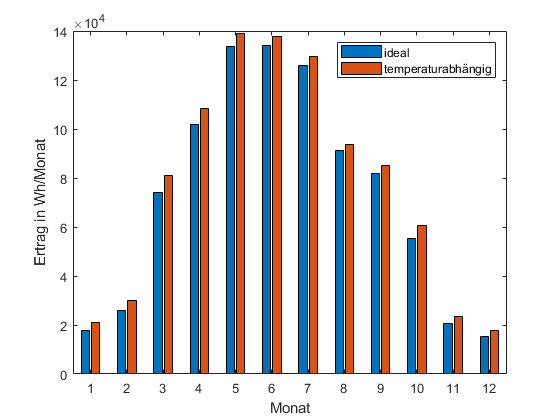
\includegraphics[width=12cm]{img/results/MonatlicheErtraegeVergleich}
		\caption{Vergleich der monatlichen Erträge der idealen und der temperaturunabhängigen Berechnung.}
	\end{figure}
	In Abbildung 2 werden die monatlichen Erträge der jeweiligen Modelle verglichen. Über das gesamte Jahr 2005 hinweg liefert das temperaturabhängige Modell einen höheren Ertrag.\newline
	In den Monaten März, April und Oktober ist die Differenz zwischen dem temperaturabhängigen und dem temperaturunabhängigen Modell am größten. Der Grund dafür ist, dass es in diesen Zeiträumen relativ kalt ist, es gleichzeitig aber mehr Einstrahlung auf die PV-Anlage gibt, als zum Beispiel in den Monaten Dezember und Jänner.
	\begin{figure}[H]
		\centering
		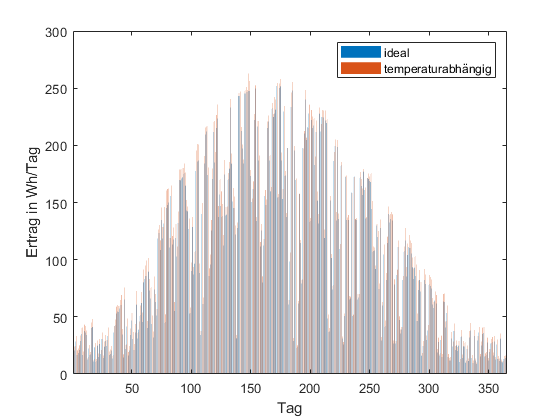
\includegraphics[width=12cm]{img/results/StuendlicheWerteVergleich}
		\caption{Vergleich der durchschnittlichen stündlichen Erträge, pro Tag, der idealen und der temperaturunabhängigen Berechnung.}
	\end{figure}
	In Abbildung 3 wird der durchschnittliche stündliche Ertrag, pro Tag, des idealen und des temperturabhängigen Modells, dargestellt. Auch in diesem Diagramm ist ersichtlich, dass der durchschnittliche stündliche Ertrag bei dem temperaturabhängigen Modell die meiste Zeit höher ist, als beim idealen Modell. Lediglich in den Sommer-Monaten von Juni bis September gibt es vereinzelt Tage, an denen das ideale Modell einen höheren Ertrag als Ergebnis hat.\newpage
	\section{Ergebnisse - Aufgabe 2.2}
	In Aufgabe 2.2. sollte die Erzeugung einer PV-Anlage, mit Standort Wien, unter Abhängigkeit des Aufstellwinkels dargestellt werden. Dazu soll der Neigungswinkel der Anlage von $0^{\circ}$ bis $90^{\circ}$ in $2.5^{\circ}$-Intervallen und der Azimut der Anlage von $0^{\circ}$ bis $360^{\circ}$ in $10^{\circ}$-Intervallen verändert werden.\newline
	Zur Berechnung soll der temperaturabhängige Ertrag verwendet werden.
	\subsection{2.2.a}
	Das Ziel von Aufgabe 2.1.a ist es der PV-Anlage in Abhängigkeit der Aufstellwinkel zu errechnen.\newline
	Hierzu wurden in MATLAB zwei Vektoren definiert:
	\begin{itemize}
		\item \textbf{pvHoehenwinkelNeu} = $0:2.5:90$.
		\item \textbf{pvAzimutNeu} = $0:10:360$
	\end{itemize}
	Mithilfe von zwei for-Schleifen kann für jede Kombination aus Azmiut und Neigungswinkel der resultierende Ertrag errechnet werden.
	\begin{lstlisting}
	for h=1:length(pvHoehenwinkelNeu)
		for a=1:length(pvAzimutNeu)
			pvModuleinfallswinkelNeu = acosd($-$cosd(sHoehenwinkel).*sind(pvHoehenwinkelNeu(h)).*cosd(sAzimut $-$ pvAzimutNeu(a)$-$180)+sind(sHoehenwinkel).*cosd(pvHoehenwinkelNeu(h)));
			[~,Eges3T] = Jahreserzeugung(pvHoehenwinkelNeu(h), pvGroesse, pvWirkungsgrad, pvVerluste, pvModuleinfallswinkelNeu, sHoehenwinkel, Strahlung, gSTC, TmodSTC, ct, Temperatur);
		end
	end
	\end{lstlisting}
	\subsection{2.2.b}
	In Aufgabe 2.2.b sollen aus dem in Aufgabe 2.2.a errechneten Ertrag, die Volllaststunden errechnet werden.\newline
	Die Volllaststunden können über die Formel
	\begin{equation}
	T=\frac{\sum \limits_{t=1}^T P_t}{P_{Peak}}
	\end{equation}
	errechnet werden.\newline
	Der MATLAB Code aus Aufgabe 2.2.a wird daher um die Berechnung der Volllaststunden erweitert.
	\begin{lstlisting}
	for h=1:length(pvHoehenwinkelNeu)
		for a=1:length(pvAzimutNeu)
			pvModuleinfallswinkelNeu = acosd($-$cosd(sHoehenwinkel).*sind(pvHoehenwinkelNeu(h)).*cosd(sAzimut$-$ pvAzimutNeu(a)$-$180)+sind(sHoehenwinkel).*cosd(pvHoehenwinkelNeu(h)));
			[~,Eges3T] = Jahreserzeugung(pvHoehenwinkelNeu(h), pvGroesse, pvWirkungsgrad, pvVerluste, pvModuleinfallswinkelNeu, sHoehenwinkel, Strahlung, gSTC, TmodSTC, ct, Temperatur);
			combinations(h,a) = sum(Eges3T)/(pvGroesse.*1000);
		end
	end
	\end{lstlisting}
	Das Ergebnis ist eine 37 x 37 Matrix, in der für jede Kombination aus Azimut und Neigungswinkel der PV-Anlage die Anzahl der Volllaststunden gespeichert ist.\newline
	Mit der Funktion $meshc$ kann aus dieser Matrix eine dreidimensionale Darstellung erstellt werden.
	\begin{figure}[H]
		\centering
		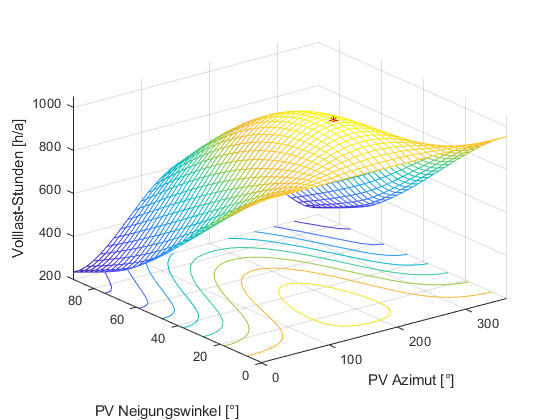
\includegraphics[width=12cm]{img/results/VolllaststundenAbhaengigVomWinkel}
		\caption{Die Anzahl der Volllaststunden in Abhängigkeit der Aufstellwinkel, der PV-Anlage.}
	\end{figure}
	Mit Hilfe der Funktion $contour$ kann eine zweidimensionale Darstellung der selben Daten erstellt werden.
	\begin{figure}[H]
		\centering
		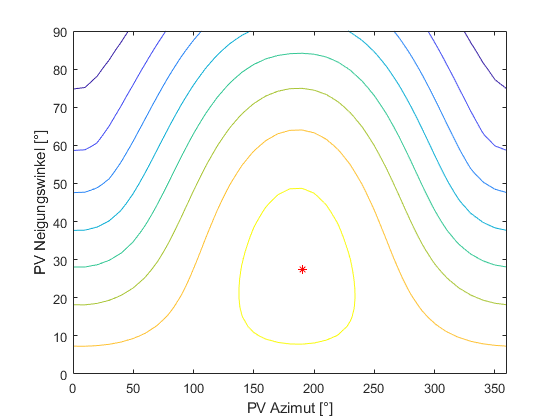
\includegraphics[width=12cm]{img/results/VolllaststundenAbhaengigVomWinkelContour}
		\caption{Die Anzahl der Volllaststunden in Abhängigkeit der Aufstellwinkel, der PV-Anlage.}
	\end{figure}
	Die maximale Anzahl an Volllaststunden (= der maximale Ertrag) wird bei einem Neigungswinkel von $27.5^{\circ}$ und einem Azimut von $190^{\circ}$ erreicht. Sie beträgt $248.5021$ Stunden. Dieser Wert wird in den Abbildungen 4 und 5 als roter Punkt dargestellt.
	\subsection{2.2.c}
	In Aufgabe 2.2.c soll die Berechnung aus Aufgabe 2.2.b spezifisch für die Monate Juni und Dezember durchgeführt werden.\newline
	Die Berechnung, sowie der MATLAB Code, kann der Beschreibung von Aufgabe 2.2.b entnommen werden.\newline
	\begin{figure}[H]
		\centering
		\begin{minipage}[b]{0.4\textwidth}
			\centering
			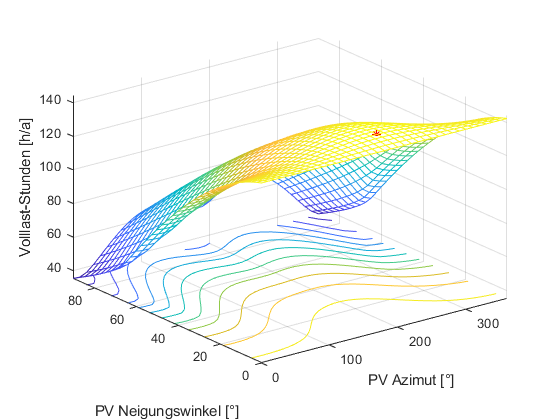
\includegraphics[width=7.5cm]{img/results/VolllaststundenAbhaengigVomWinkelJuni}
		\end{minipage}
		\hfill
		\begin{minipage}[b]{0.4\textwidth}
			\centering
			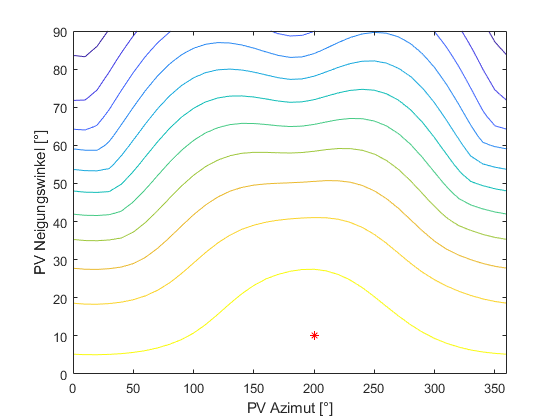
\includegraphics[width=7.5cm]{img/results/VolllaststundenAbhaengigVomWinkelContourJuni}
		\end{minipage}
		\caption{Die Anzahl der Volllaststunden in Abhängigkeit der Aufstellwinkel, der PV-Anlage, für das Monat Juni.}
	\end{figure}
	\begin{figure}[H]
		\centering
		\begin{minipage}[b]{0.4\textwidth}
			\centering
			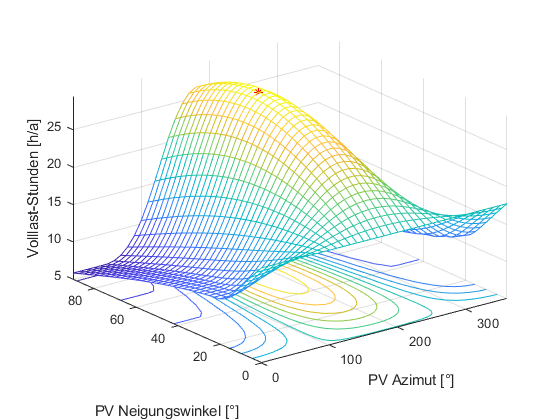
\includegraphics[width=7.5cm]{img/results/VolllaststundenAbhaengigVomWinkelDezember}
		\end{minipage}
		\hfill
		\begin{minipage}[b]{0.4\textwidth}
			\centering
			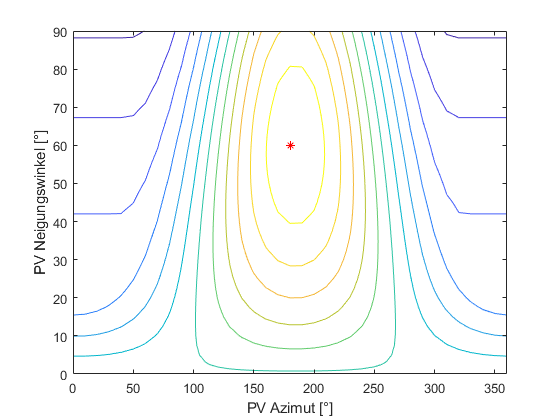
\includegraphics[width=7.5cm]{img/results/VolllaststundenAbhaengigVomWinkelContourDezember}
		\end{minipage}
		\caption{Die Anzahl der Volllaststunden in Abhängigkeit der Aufstellwinkel, der PV-Anlage, für das Monat Dezember.}
	\end{figure}
	In den Abbildungen 6 und 7 werden die Volllaststunden, bei veränderten Aufstellwinkeln der PV-Anlage, dargestellt. Der jeweils maximale Ertrag wird durch einen roten Punkt gekennzeichnet.\newline
	Die optimalen Aufstellwinkel lauten:
	\begin{table}[H]
		\centering
		\begin{tabular}{|c|c|c|c|}
			\hline
			& Azmiut        & Neigungswinkel & Kommentar                                                                                                                                                                        \\ \hline
			Juni     & $200^{\circ}$ & $12.5^{\circ}$ & \begin{tabular}[c]{@{}c@{}}Die Sonne steht im Juni zur Mittagszeit fast senkrecht\\  auf den Horizont\\ =\textgreater flacher optimaler Neigungswinkel der Anlage\end{tabular} \\ \hline
			Dezember & $180^{\circ}$ & $60^{\circ}$   & \begin{tabular}[c]{@{}c@{}}Der Sonnenweg ist im Dezember sehr flach\\ =\textgreater steiler optimaler Neigungswinkel der Anlage\end{tabular}                                     \\ \hline
		\end{tabular}
	\end{table}
	\section{Ergebnisse - Aufgabe 2.3}
	Zusätzlich zu den Aufstellwinkeln der PV-Anlage ist der Standort dieser maßgeblich entscheidend für den Ertrag.\newline
	In Aufgabe 2.3 sollten zusätzlich zu der PV-Anlage in Wien zwei weitere Standorte in Europa ausgewählt werden.\newline
	Die zusätzlichen zwei Standorte sind in unserem Fall:
	\begin{table}[H]
		\centering
		\begin{tabular}{|c|c|c|}
			\hline
			& Längengrad         & Breitengrad        \\ \hline
			Neapel & $14.24878^{\circ}$ & $40.83593^{\circ}$ \\ \hline
			London & $-0.12765^{\circ}$ & $51.50732^{\circ}$ \\ \hline
		\end{tabular}
	\end{table}
	\subsection{2.3.a}
	In Aufgabe 2.3.a sollten die drei Standorte verglichen werden. Der Vergleich erfolgt aufgrund der gesamten Jahreserzeugung, der Volllaststunden und der durchschnittlichen Tagesproduktion.\newline
	Für die folgenden Berechnungen ist der Azimut für alle Standorte $270^{\circ}$ und der Neigungswinkel $20^{\circ}$.\newline
	Die gesamte Jahresproduktion, sowie die Volllaststunden der drei Standorte, werden in folgender Tabelle dargestellt.
	\begin{table}[H]
		\centering
		\begin{tabular}{|c|c|c|}
			\hline
			& \begin{tabular}[c]{@{}c@{}}Gesamte Jahresproduktion\\  (in Wh)\end{tabular} & Volllaststunden \\ \hline
			Wien   & $1.8881e+05$                                                                & $188.8145$      \\ \hline
			Neapel & $1.4019e+06$                                                                & $1401.9$        \\ \hline
			London & $8.7242e+05$                                                                & $872.4218$      \\ \hline
		\end{tabular}
	\end{table}
	Die gesamte Jahresproduktion und somit auch die Anzahl der Volllaststunden, ist in Neapel am höchsten. Da Neapel der südlichste der drei Standorte ist, war dies zu erwarten. Zusätzlich wird die Temperatur in der Berechnung nicht berücksichtigt, was den Ertrag in Neapel noch höher wirken lässt. In der Realität müsste man natürlich die Temperatur in die Berechnung miteinbeziehen.\newline
	\begin{figure}[H]
		\centering
		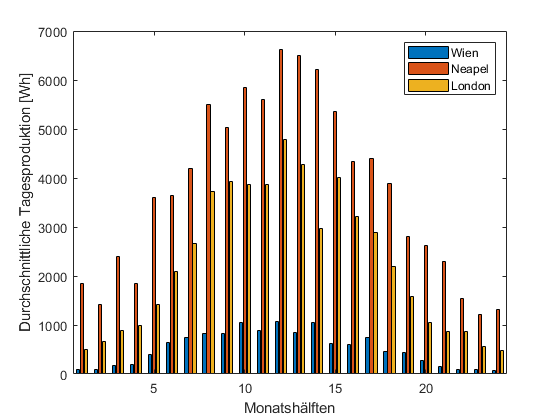
\includegraphics[width=12cm]{img/results/StandortVergleichTagesproduktion}
		\caption{Die durchschnittliche Tagesproduktion der Standorte Wien, Neapel und London.}
	\end{figure}
	In Abbildung 8 wurde für die drei Standorte die durchschnittliche Tagesproduktion errechnet. Auch hier ist der Ertrag in Neapel am höchsten.
	\subsection{2.3.b}
	Das Ziel von Aufgabe 2.3.b war es die optimalen Aufstellwinkel der beiden zusätzlichen Standorte zu identifizieren.\newline
	Die Berechnung sowie der MATLAB Code wird in Aufgabe 2.2 beschrieben.
	\begin{figure}[H]
		\centering
		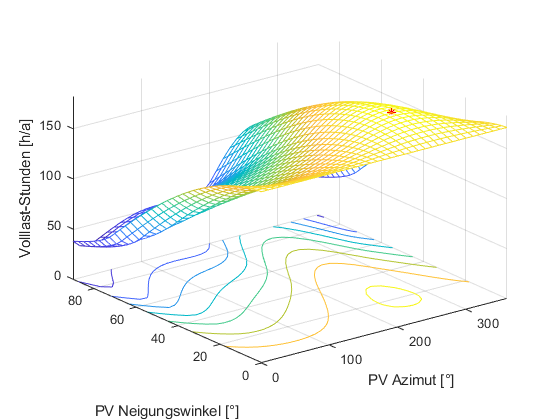
\includegraphics[width=12cm]{img/results/VolllaststundenAbhaengigVomWinkelNeapel}
		\caption{Die Anzahl der Volllaststunden in Abhängigkeit der Aufstellwinkel, einer PV-Anlage mit Standort Neapel.}
	\end{figure}
	Für den Standort \textbf{Neapel} ergibt sich ein optimaler Azimut von $260^{\circ}$ und ein optimaler Neigungswinkel von $22.5^{\circ}$. Die Volllaststunden sind damit $181.3758$.
	\begin{figure}[H]
		\centering
		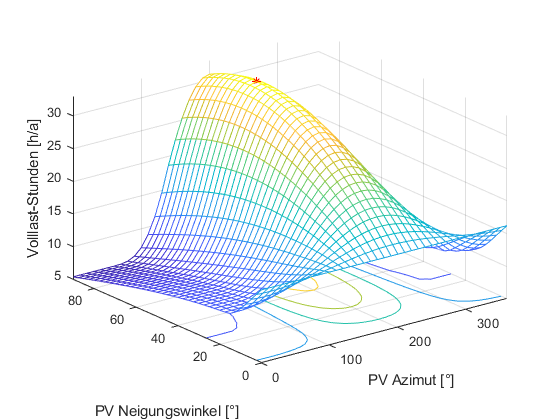
\includegraphics[width=12cm]{img/results/VolllaststundenAbhaengigVomWinkelLondon}
		\caption{Die Anzahl der Volllaststunden in Abhängigkeit der Aufstellwinkel, einer PV-Anlage mit Standort London.}
	\end{figure}
	Für den Standort \textbf{London} ergibt sich ein optimaler Azimut von $200^{\circ}$ und ein optimaler Neigungswinkel von $67.5^{\circ}$. Die Volllaststunden sind damit $33.0063$.\\ \par
	Analog zu der Abhängigkeit der Volllaststunden von der Jahreszeit, kann man auch bei den Standorten erkennen, dass bei einer Einstrahlung, die fast senkrecht zum Horizont ist, ein geringer Neigungswinkel vorteilhaft ist. Dies ist bei Standorten, die nahe am Äquator liegen, der Fall.\newline
	London ist weiter vom Äquator entfernt, weshalb der Einstrahlungswinkel nicht sehr steil ist, wodurch wiederum ein höherer Neigungswinkel der PV-Anlage optimal ist.
	\subsection{2.3.c}
	In Aufgabe 2.3.c soll begründet werden, warum die Erzeugung aus PV-Anlagen an unterschiedlichen Standorten zeitliche (tageszeitliche und saisonal) Unterschiede aufweist.\newline
	Die Begründung hierfür heißt "Lichter Tag". Der lichte Tag beschreibt die Zeitspanne von Sonnenaufgang bis Sonnenuntergang.\newline
	Die Tageslänge ist vor allem von der geografischen Breite des Standortes abhängig. Abseits des Äquators dauert der lichte Tag, in Relation zur Nacht, unterschiedlich lange. Dieser Effekt ist der Neigung der Erde geschuldet.\newline
	Generell gilt, je weiter der Breitengrad des Standortes vom Äquator entfernt ist, desto größer sind die jahreszeitlichen Unterschiede zwischen Tag und Nacht.\newline
	Umso näher man den Polen kommt, umso extremer ist das Tag/Nacht Verhältnis. (siehe Abbildung 11)\newline
	\begin{figure}[H]
		\centering
		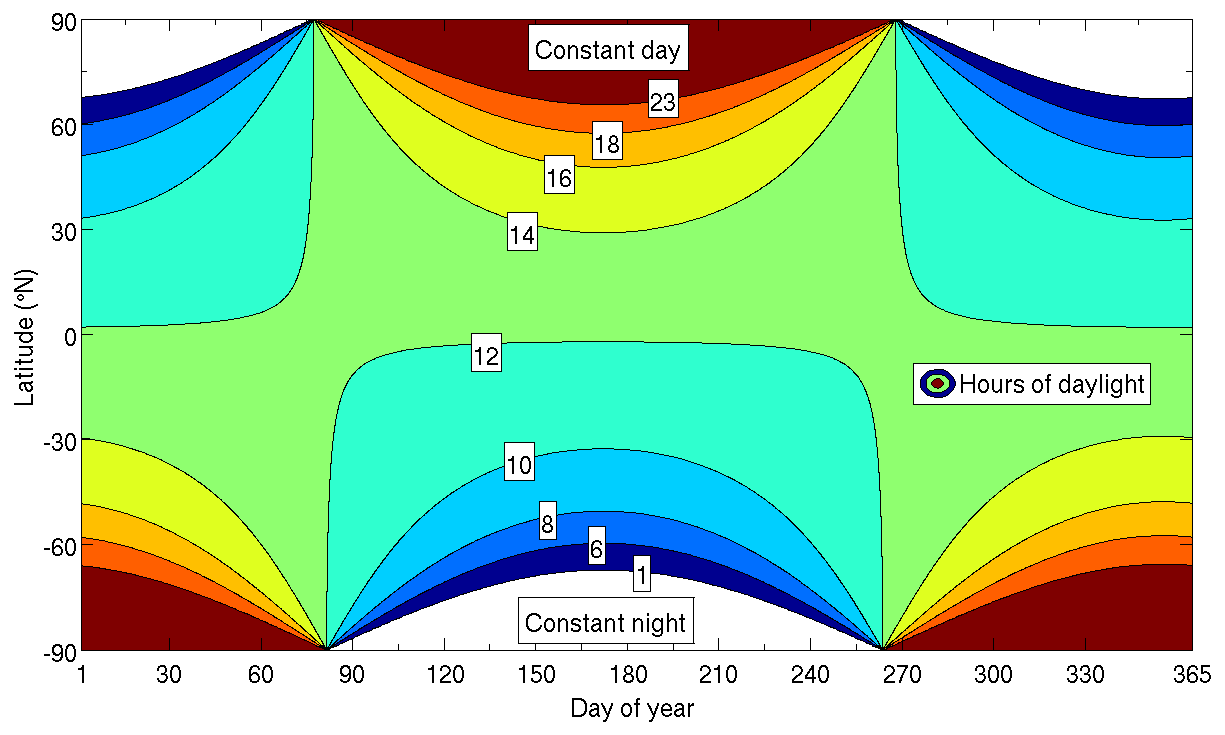
\includegraphics[width=12cm]{img/results/LichtTagDauer}
		\caption{Die Dauer des lichten Tags in Stunden, in Abhängigkeit von der geografischen Breite. Quelle: Wikipedia}
	\end{figure}
	Im Sommer sind die Tage, nahe dem Nordpol, zwar lange, dafür ist die Einstrahlung aufgrund des Einfallwinkels nicht stark. Auf der anderen Seite sind die Tage im Sommer, nahe dem Südpol, sehr kurz. Dadurch entstehen die saisonalen Unterschiede.\newline
	Durch die unterschiedliche Dauer des lichten Tages ändert sich auch der Verlauf der Einstrahlung zwischen Sonnenaufgang und Sonnenuntergang. (und damit auch die Erzeugung) Dadurch entstehen die tageszeitlichen Unterschiede.
	\newpage
	\section{Literatur}
	\begin{itemize}
		\item Modellierung eines Wärmeschichtspeichers mit
		Solareinbindung in Excel/VBA von Rainer Blabensteiner
		\item Mapping the performance of PV modules, effects of module type and data averaging von Thomas Huld, Ralph Gottschalg, Hans Georg Beyer und Marko Topic
	\end{itemize}
	\newpage
	\listoffigures
\end{document}